\documentclass[conference]{IEEEtran}
\IEEEoverridecommandlockouts
% The preceding line is only needed to identify funding in the first footnote. If that is unneeded, please comment it out.
\usepackage{cite}
\usepackage{amsmath,amssymb,amsfonts}
\usepackage{algorithmic}
\usepackage{graphicx}
\usepackage{textcomp}
\usepackage{pdfpages}
\usepackage{xcolor}
\usepackage{svg}
\usepackage{float}
\usepackage{hyperref}
\usepackage{url}
\usepackage{graphicx}
\usepackage{dblfloatfix}

\hypersetup{
    colorlinks,
    citecolor=black,
    filecolor=black,
    linkcolor=black,
    urlcolor=black
    pdftitle={EE300 İsmail Enes Bülbül}
}

\def\BibTeX{{\rm B\kern-.05em{\sc i\kern-.025em b}\kern-.08em
    T\kern-.1667em\lower.7ex\hbox{E}\kern-.125emX}}

\begin{document}

\title{EE 313 ANALOG ELECTRONICS LABORATORY 2022-2023 FALL TERM PROJECT REPORT \\ {\large AN OPTICAL WIRELESS COMMUNICATION SYSTEM: PHOTOPHONE}}

\author{\IEEEauthorblockN{Ahmet Caner Akar}
\IEEEauthorblockA{\textit{Electrical and Electronics Engineering Department} \\
\textit{Middle East Technical University}\\
Ankara, Turkey \\
e244228@metu.edu.tr}
\and
\IEEEauthorblockN{İsmail Enes Bülbül}
\IEEEauthorblockA{\textit{Electrical and Electronics Engineering Department} \\
\textit{Middle East Technical University}\\
Ankara, Turkey \\
e244263@metu.edu.tr}
\and
}

\maketitle

\begin{abstract}
This document is about the end-term project of EE313 Analog Electronics Laboratory, namely design of an optical wireless communication system: photophone. Background theoretical knowledge, literature research and various work about design methods and mathematical analysis of them related to this project together with simulation and experimental results are defined in this document. \\
\end{abstract}

\begin{IEEEkeywords}
Optical wireless communication, freespace optical communication, Li-Fi, photophone, AGC, laser
\end{IEEEkeywords} 

\section{Introduction}
Communication is an integral part of our lives for us humans, who are social beings. While it was carried out by methods such as pigeons or fire in history, various types of communication have emerged with the advancement of technology. In this project, we will examine the one of the modern communication systems: optical wireless communication system. The overall diagram of the project is given in Fig. 1, below for better understanding.
\begin{figure}[H]
   \centerline{\includesvg[inkscapelatex=false, scale=0.25]{devre}}
    \caption{Overall block diagram of the system}
\end{figure}
 \par The aim of the project is to transmit the audio input signal that is generated by the microphone and to receive this information wirelessly. Then, the received signal is fed to the speaker at the final step while the quality of the signal is indicated by a single RGB LED. In general, the project can be grouped under two main units: Transmitter Unit and Receiver Unit, as it can be seen in Fig. 1. Also, each main part consists of different sub-units, and they are explained in detail in the following sections of the report.
\section{Rules}
\noindent Maximum allowed DC Voltage: ±15 Volts. \\
Instruments not allowed using: 6V terminal of the DC supply.\\ 
Frequency Range for Reference Signal: 10 kHz – 30 kHz. \\
Component not allowed to be used: audio op-amps, microphone with integrated driving circuitries, infrared and ultraviolet lasers, and visible light lasers whose power \(>\) 5mW.
\section{Transmitter Unit}
\subsection{Microphone Driver}
The first part of the transmitter unit is microphone driver circuit. To transmit an audio signal using a laser, we need to detect this audio signal first. Therefore, to do this we used an electret microphone. It requires a biasing voltage to operate. Thus, we biased the microphone by connecting the positive terminal of it to the 1 k\(\Omega\) resistor. However, since the output voltage of the microphone is quite low, we cannot directly connect it to the rest of the circuit. In order to use this output, first, we should amplify it with a non-inverting amplifier circuit as shown in Fig. 2. 
 \begin{figure}[H]
   \centerline{\includesvg[inkscapelatex=false, scale=0.25]{microphone}}
    \caption{Microphone driver circuit schematic}
\end{figure}
 \par There is a 10 k\(\Omega\) potentiometer connected between ground and the inverting input of the amplifier so that by changing its value, the gain can be adjusted, and the amplitude of the output signal is changed. The gain of the topology can be found by the following expression (1).
\begin{equation}\label{eq:1}
        Gain, A_v = \frac{R_3+R_4}{R_4} 
 \end{equation}
\par Also, the simulation result of the input-output characteristics of the microphone driving circuit in LTspice is given in Fig. 3 when R\(_4\) = 10k\(\Omega\).
 \begin{figure}[H]
   \centerline{\includesvg[inkscapelatex=false, scale=0.25]{microphone_driver_1}}
    \caption{Microphone driver circuit, simulation result}
\end{figure}
\par The experimnental result of the microphone driver circuit when 1 kHz sine tone is played from mobile phone can be seen in Fig. 4, and we can say that the experimental and simulation results are similar to each other. 
 \begin{figure}[H]
   \centerline{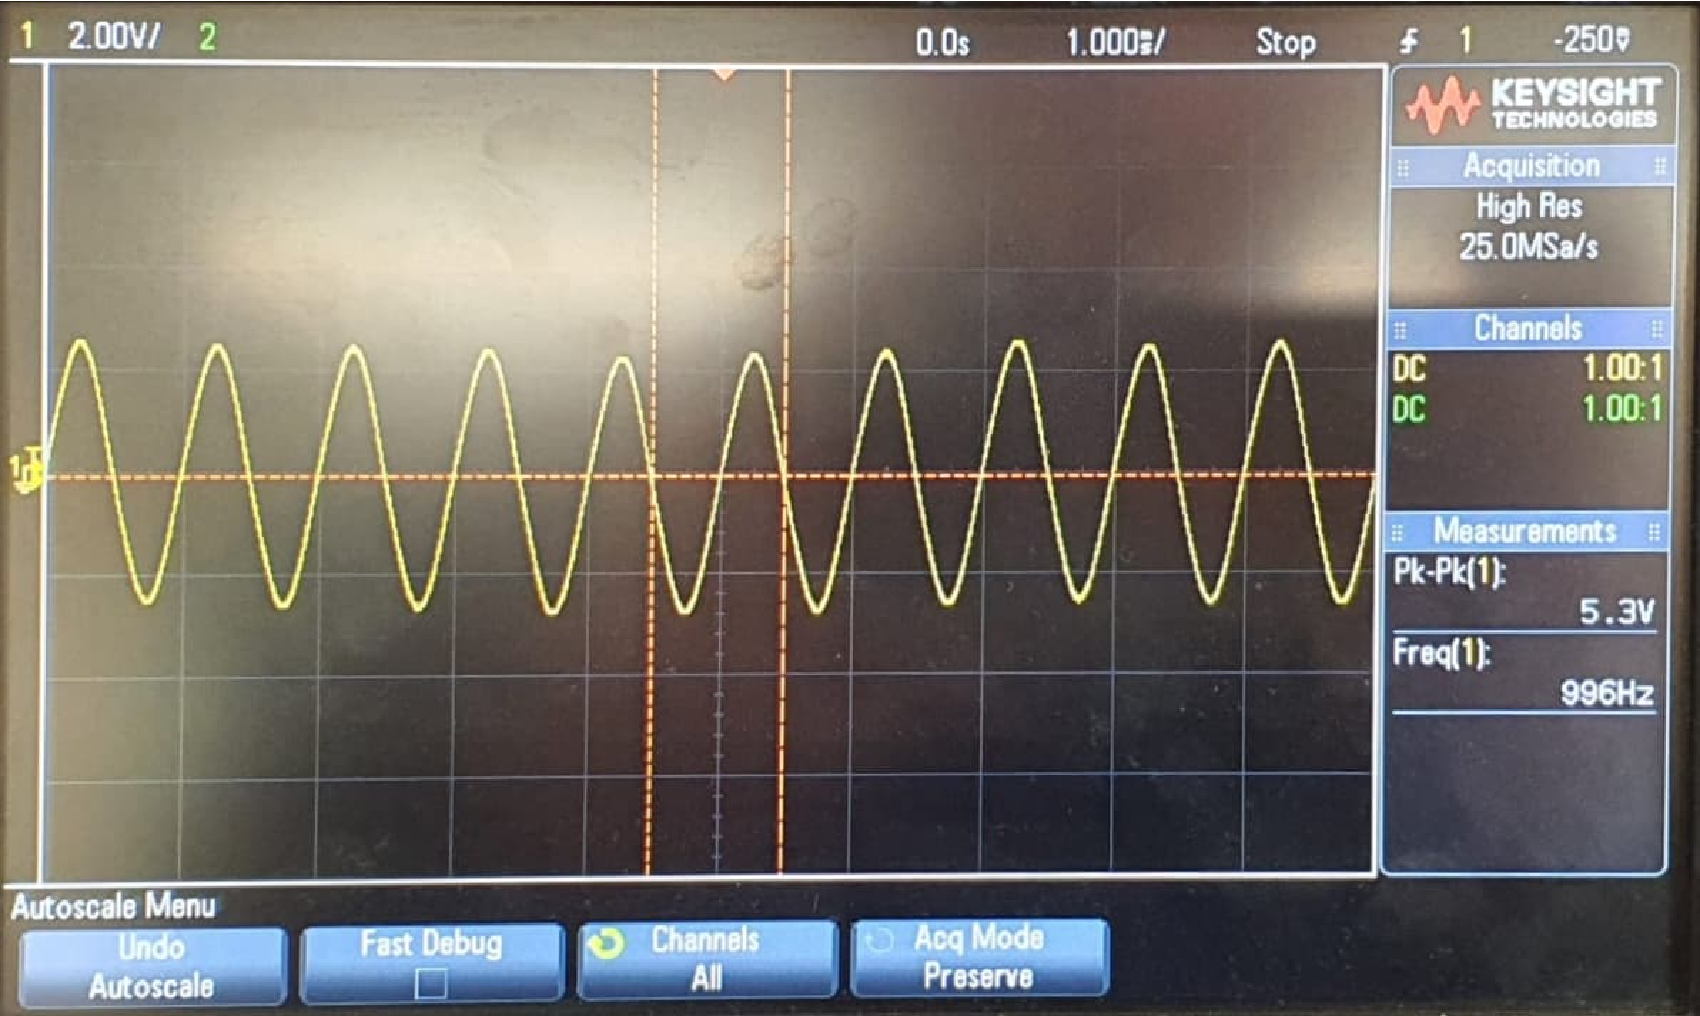
\includegraphics[scale=0.13]{microphone.png}}
    \caption{Microphone driver circuit, experimental result}
\end{figure} 
\par After non-inverting amplifier circuit, we connected a buffer circuit so that the microphone driver will not be affected from the rest of the circuit. 
\subsection{Automatic Gain Control}
The second sub-unit of the transmitter part is Automatic Gain Control (AGC). We should adjust the output signal of the microphone driver circuit because the output of the microphone is distance and frequency dependent, so the output amplitude of the microphone change with time as well as distance of the speaker (person) to it. Therefore, as it is stated in project definition, we need an automatic gain controller that controls gain and adjusts the amplitude of the microphone signal so that we will get a relatively constant amplitude audio signal at the output of the AGC regardless of the amplitude of the input signal. To achieve this, we construct the AGC circuit which can be seen in Fig. 5.
 \begin{figure}[H]
   \centerline{\includesvg[inkscapelatex=false, scale=0.25]{agc}}
    \caption{Automatic Gain Control circuit schematic}
\end{figure}
\par In fact, the AGC circuit in Fig. 5 is a negative feddback amplifier topology. The upper part of the circuit is basically a non-inverting amplifier whereas the remaining part is feedback network. The output of the microphone driver circuit is connected to the non-inverting input of the op-amp, and it is amplified by the gain of the amplifier which is determined by the resistors connected to the inverting input (2). 
\begin{equation}\label{eq:2}
        Gain, A_v = \frac{R_7+R_8}{R_7} 
 \end{equation}
\par At the output of the op-amp, a diode, resistor and capacitor is connected in series. Actually, it is a basic peak detector, and it is used to detect the peak voltage value of the output of the op-amp. Here, we used 1N4148 fast diode \cite{1N4148} since the change in the audio signal is generally fast. Then, the output of the peak detector is used to bias the BC547 NPN transistor so that the collector current is passing through the 100 k\(\Omega\) resistor, and the voltage exists at the gate terminal of the 2N5460 JFET. Thus, as the amplitude of the input signal is changed the voltage at the gate terminal of the JFET is also changed. Also, since JFET can be used as a voltage controlled resistor, the voltage at the non-inverting of the op-amp is changed as well. So, this is how the negative feedback works in the AGC part. As a result, we get almost a constant amplitude signal at the output of the AGC regardless of the amplitude of the input signal. The simulation result of the AGC can be seen in Fig. 6 which shows output values for a 2 kHz sine wave with different amplitudes.
 \begin{figure}[H]
   \centerline{\includesvg[inkscapelatex=false, scale=0.25]{new_agc_jfet}}
    \caption{Automatic Gain Control circuit, simulation result}
\end{figure}
\subsection{Low-Pass Filter}
Although the frequency range of human voice is from 80 Hz to 14 kHz, in the project definition it is stated that the system only uses the portion of 300 Hz to 3.4 kHz. Therefore, we connected the output of the AGC to a low-pass filter before the addition of the high-frequency reference signal, so that the audio signal and the reference signal does not overlap in frequency spectrum. For filtering process, we utilized a \(4^{th}\) order Butterworth low-pass filter whose cut-off frequency can be found by (4). 
\begin{equation}\label{eq:a}
f_c = \frac{1}{2\pi RC}
\end{equation}  
\par The circuit schematic of our low-pass fiter is shown in Fig. 7.  Also, the simulation result of AC analysis of the low-pass filter in LTspice is given in Fig. 8.
 \begin{figure}[H]
   \centerline{\includesvg[inkscapelatex=false, scale=0.25]{lpf}}
    \caption{Low-Pass filter circuit schematic}
\end{figure}
 \begin{figure}[H]
   \centerline{\includesvg[inkscapelatex=false, scale=0.25]{lpf_result}}
    \caption{Low-Pass filter circuit, AC analysis simulation result}
\end{figure} 
\subsection{Summing Amplifier}
Before transmitting the audio signal, we are going to add another signal namely reference signal so that at the receiver side, the amplitude of this signal will be treated as the measure of signal strength since it is constant. To sum up these two signals, we used a basic summing amplifier circuit which can be seen in Fig. 9.
 \begin{figure}[H]
   \centerline{\includesvg[inkscapelatex=false, scale=0.25]{summing_amplifier}}
    \caption{Summing amplifier circuit schematic}
\end{figure} 
\par For the summing amplifier the output expression can be given as by the following equation (4). The output voltage has \(180^\circ\) phase shift since the audio and reference signals are given from the inverting input of the op-amp.  
\begin{equation}\label{eq:3}
         V_{out} = -\frac{R_3}{R_1} \mbox{(Audio\textunderscore signal)} - \frac{R_3}{R_2} \mbox{(Reference\textunderscore signal)}
 \end{equation}
 \par The simulation result of the summing amplifier in LTspice is shown in Fig. 10. Also, the experimental result of the summing amplifier when we played 1 kHz sine tone from mobile phone can be seen in Fig. 11. From the figures, we can conclude that the transmitter unit from beginning to summing amplifier ouput works 
 quite well.  
  \begin{figure}[H]
   \centerline{\includesvg[inkscapelatex=false, scale=0.25]{summing_amplifier_1}}
    \caption{Summing amplifier, simulation result}
\end{figure} 
 \begin{figure}[H]
   \centerline{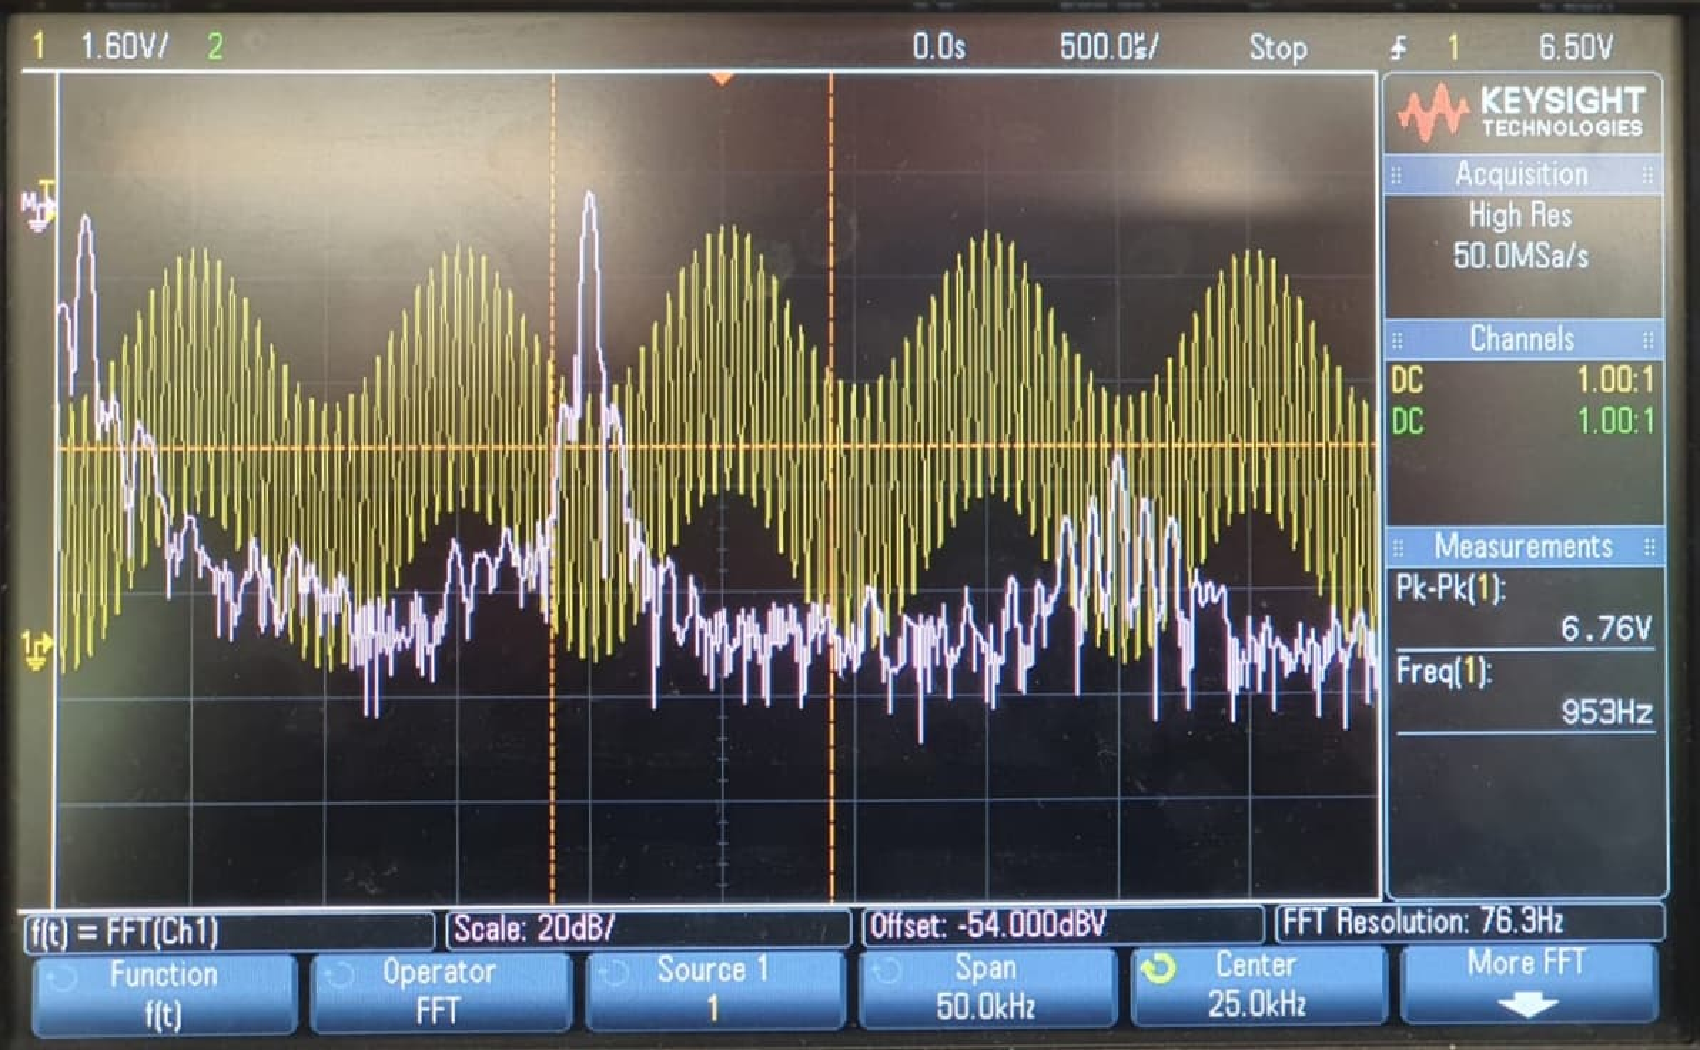
\includegraphics[scale=0.13]{summing.png}}
    \caption{Summing amplifier circuit, experimental result}
\end{figure} 
 \par In the summing amplifier circuit, we did not use a regular op-amp such as LM741 or UA741. Since we are working with high frequencies, we had to use an opamp with higher slew-rate for better response. Thus, we used an LF351 \cite{LF351} opamp which has a slew rate of 16V/\(\mu\)s whereas LM741 \cite{LM741} and UA741 \cite{uA741} op-amps has a slew rate of 0.5V/\(\mu\)s.
\subsection{Laser Driver}
At the transmitter unit, we need to convert the electrical signal to modulated light signal. To achieve this, we decided to use a laser rather than infrared or visible light LEDs because the visible light LEDs are very sensitive to the environmental noise whereas the infrared LEDs are not observable by naked eye so that it is hard to check whether the system works properly. \\ 
\par The light intensity of lasers is somewhat linearly dependent on the current, not the voltage as it can be seen from Fig. 12.
 \begin{figure}[H]
   \centerline{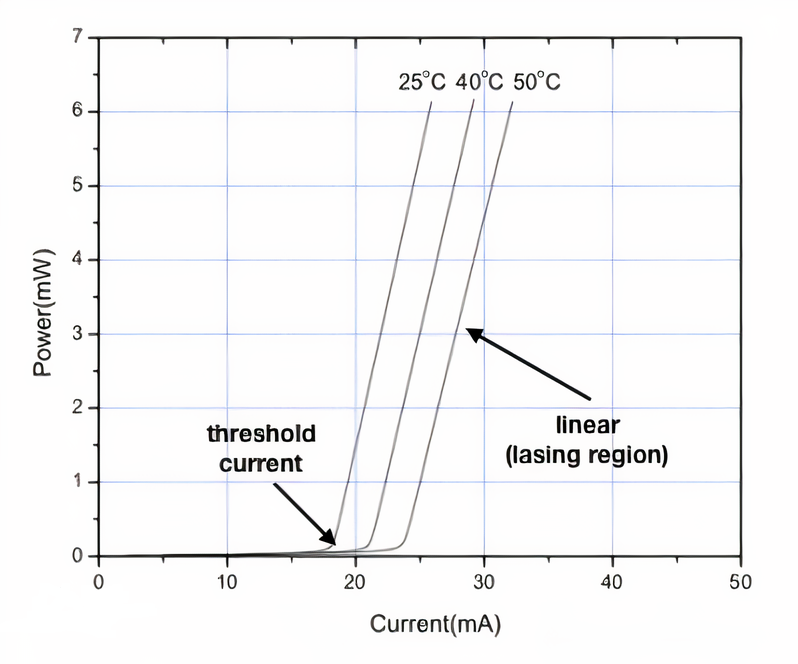
\includegraphics[scale=0.5]{laser.png}}
    \caption{Current–light intensity characteristics of typical laser diode}
\end{figure} 
\par Therefore, the laser drive circuit is a transconductance amplifier whose input voltage coming from the summing amplifier, and the circuit schematic is shown in Fig. 13.
 \begin{figure}[H]
   \centerline{\includesvg[inkscapelatex=false, scale=0.25]{laser}}
    \caption{Laser driver circuit schematic}
\end{figure} 
\par In this circuit, we utilizied the BC557 PNP transistor to construct a common-emitter amplifier with degeneration. As seen in Fig. 12 the light intensity of the laser is linear after some threshold current, which is also called as linear region. Thus, we want laser to operate in this region, so we need some kind of DC current offset. To achieve this, the resistors R2 and R3 is connected to the base terminal of the transistor so that the DC voltage at the base terminal is approximately equal to 7.5 V. Also, the simulation result of the DC operating point of the transistor can be seen in Fig. 14. 
 \begin{figure}[H]
   \centerline{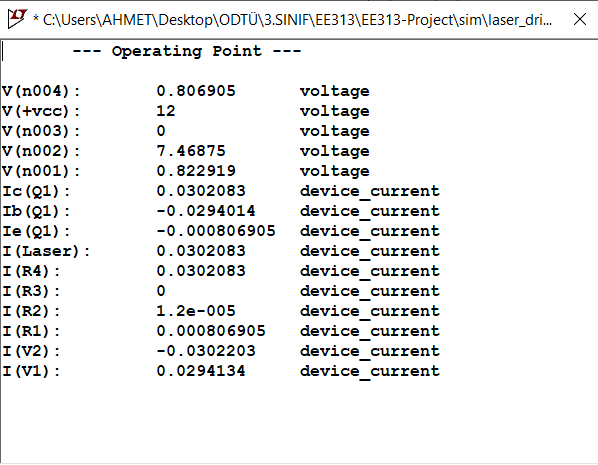
\includegraphics[scale=0.5]{DC_operating.png}}
    \caption{DC operating point of the transistor, simulation result}
\end{figure} 
\par It can be seen from Fig. 14 that DC current of the collector terminal, Ic(Q1) \(\thickapprox \) 30 mA. This value is enough to operate the laser in linear region. In this topology, we feed our signal from base terminal of the transistor, so we have a better small signal range. Also, we connected a degeneration resistor at emitter terminal of the transistor. Although the degeneration resistor decreases the gain, it improves small-signal range and provides staility to circuitry. Also, we connected 220 \(\Omega\) resistor to the collector terminal because the maximum allowed operating voltage of the laser is about 6V otherwise it may be damaged. The simulation result of the laser driver circuit is shown in Fig. 15.  
 \begin{figure}[H]
   \centerline{\includesvg[inkscapelatex=false, scale=0.25]{laser_driver_new_1}}
    \caption{Laser driver circuit, simulation result}
\end{figure} 

\section{Receiver Unit}
\subsection{Photodiode}
At the beginning of the receiver, we need to obtain light and convert it to a voltage signal. To do this, we decided to use the BPW34 photodiode \cite{BPW34} 
since it operates at visible light. The photodiode is a device which has a current changing with light on the device, so that we can use it 
to convert light into current. At this stage we decided to use a transimpedance amplifier to convert current to voltage. The schematic of the amplifier 
is shown in Fig. 16, below.
%% SCHEMATIC.
\begin{figure}[H]
  \centerline{\includesvg[inkscapelatex=false, scale=0.25]{diode}}
  \caption{The schematic of the photodiode driving circuit}
\end{figure} 


\subsection{Low-Pass and High-Pass Filter}
After the light signal is converted to voltage signal, we need to seperate the audio and the reference signal. We need to implement 
a low-pass filter to obtain the audio signal and a high-pass filter to obtain the reference signal. We decided to use 4\(^{th}\) order Butterworth 
Filter \cite{butterworth} for low-pass filter and 2\(^{nd}\) order Butterworth Filter for high-pass filter. The schematics of the filters are shown in Fig. 17 and Fig. 18, below. 
%% SCHEMATICs
\begin{figure}[H]
   \centerline{\includesvg[inkscapelatex=false, scale=0.25]{lpf}}
    \caption{The schematic of the low-pass filter}
\end{figure}
\begin{figure}[H]
   \centerline{\includesvg[inkscapelatex=false, scale=0.25]{hpf}}
    \caption{The schematic of the high-pass filter}
\end{figure}


The 4.7 k\(\Omega\) and 10 k\(\Omega\) resistors are for amplifying the signal. The 33 k\(\Omega\) resistors and capacitors are used to filter the signal. 
The cut-off frequency can be calculated by (3).

The frequency responses of the filters are shown in Fig. 19 and Fig. 20, below. 
%% RESULTS
\begin{figure}[H]
   \centerline{\includesvg[inkscapelatex=false, scale=0.25]{lpf_result}}
    \caption{The simulation result of the low-pass filter}
\end{figure}
\begin{figure}[H]
   \centerline{\includesvg[inkscapelatex=false, scale=0.25]{hpf_result}}
    \caption{The simulation result of the high-pass filter}
\end{figure}

From the frequency responses obtained in the simulation, we can see that low-pass filter has a bandwidth that includes 300Hz-3.4kHz and filters 20kHz. 
Similarly, 20kHz can pass through high-pass filter and low frequency components are filtered. 

\subsection{Improved Peak Detector}
At the proposal report, we decided to use a simple circuit with one diode and one capacitor to obtain the amplitude 
of the reference signal and it worked properly at the simulations. However, in practical case, it did not work as we expected 
since the frequency (20kHz) of the signal is too high. Therefore, we changed our design and used the circuit shown in \cite{peak}, and it can be seen in Fig. 21, below.
%% SCHEMATIC
\begin{figure}[H]
   \centerline{\includesvg[inkscapelatex=false, scale=0.25]{peak_detector}}
    \caption{The circuit schematic of the peak detector circuit}
\end{figure}
\par Also, the simulation result for the peak detector circuit is shown in Fig. 22.
%% RESULTS
\begin{figure}[H]
   \centerline{\includesvg[inkscapelatex=false, scale=0.25]{peak_detector_1}}
    \caption{The simulation result of the peak detector circuit}
\end{figure}

From the results, we can see that the circuit is able to get amplitude of the referance signal with high frequency.

\subsection{Signal Level Indicator}
We are expected to design a circuit to represent received signal level with a single RGB led. Chosen colors for 
each case are shown in Table 1, below.
\begin{table}[htbp]
    \caption{Led colors for each case}
    \begin{center}
    \begin{tabular}{|c|c|c|c|c|}
    \hline
    \textbf{Signal Level} & \textbf{Color}& \textbf{R Pin}& \textbf{G Pin}& \textbf{B Pin} \\
    \hline
    No Signal & - & 0 & 0 & 0\\
    \hline
    Weak Signal & Red & 1 & 0 & 0\\
    \hline
    Moderate Signal & Yellow & 1 & 1 & 0\\
    \hline
    Good Signal & Green & 0 & 1 & 0\\
    \hline
    No Signal & Blue & 0 & 0 & 1\\
    \hline
    \end{tabular}
    \label{tab1}
    \end{center}
\end{table}
\par The overall schematic of the signal level indicator circuit is shown below.
% SCHEMATIC
\begin{figure}[H]
   \centerline{\includesvg[inkscapelatex=false, scale=0.25]{window_comparator}}
    \caption{The circuit schematic of the signal level indicator}
\end{figure}
\par At first, we used 5 resistors connected in serial between Vcc and ground to divide Vcc into four different voltages 
to determine regions for each signal level case. 
Then four comparator is used to determine at which region the amplitude of the reference signal is. When the amplitude 
is at the first region, all comparators will have negative output and no color will be displayed. When the amplitude 
is at the second and third region, the first and the second comparator will have a positive output and red and yellow 
color will be displayed respectively. The output of the third comparator is substracted from the output of the first 
comparator by the difference amplifier so that the red pin will be turned off when the signal is at the fourth region 
and green color will be displayed. Similarly, the output of the last comparator is substracted from the output of the 
second comparator so that the green pin will be turned off and blue color will be displayed when the amplitude is at the 
last region.

\par We used common anode RGB led so that the led has a common ground pin. We used different resistors for each color pin of the led 
to adjust the tone of the colors. 

\par The simulation results are shown below.
%% RESULTS
\begin{figure}[H]
    \centerline{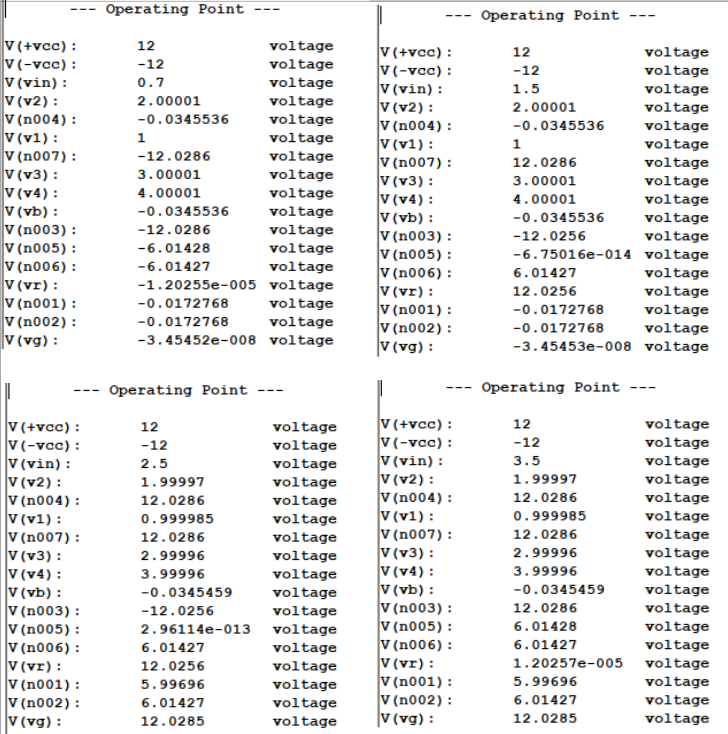
\includegraphics[scale=0.4]{wcr.png}}
     \caption{Window comparator, experimental result}
 \end{figure} 
\par From the results, we can see that for signals with different amplitude, we can see that the the red color (Vr) can be displayed at 
a specific voltage range. Therefore, we can say that the circuit is able to display 4 distinct colors for different voltage ranges. 

\subsection{Audio Amplifier}
\par We obtained the audio signal at the output of the low-pass filter. But since it has a high output resistance, we cannot directly connect 
the speaker to the output of the low-pass filter. Therefore, we need to implement a power amplifier circuit. The schematic of the power 
amplifier is shown below. 
%% SCHEMATIC
\begin{figure}[H]
   \centerline{\includesvg[inkscapelatex=false, scale=0.25]{speaker}}
    \caption{The circuit schematic of the audio amplifier}
\end{figure}
\par We are expected to deliver at least 5W power to the speaker. The power of the speaker can be calculated by (x)
\begin{equation}
    P = \frac{V^2}{R}
\end{equation}
\par We use a speaker which has 8 \(\Omega\) internal resistance. Therefore, by (x), the output of the signal should be at least 8 Vpp. The 
simulation results of the circuit is shown below. 
%% SIM RESULTS
\begin{figure}[H]
   \centerline{\includesvg[inkscapelatex=false, scale=0.25]{speaker_result}}
    \caption{The simulation result of the audio amplifier}
\end{figure}
\par From the simulation results, we can see that a sinusoidal signal with 4.5V amplitude. Therefore, we can say that the circuit can deliver 
1W power to the spekaer. In practice, however, our circuit is not worked as we expected since the BJTs we use has a current limit and burn 
at that current. Therefore, we could deliver a pretty less power and the audio can be heard from much small distance. 
\section{Conclusion}
In this project, we tried to satisfy the desired task by suggesting our solution with circuit representations and their simulation results in LTspice. During the project we tried to put the knowledge that we learned in EE313 and EE311 courses, into practice. However, sometimes it is not sufficient to solve problems based on our prior knowledge so that it necessary to do research to solve problems. Thus, we also learned how to do research and implement something that we found by considering our requirement. \\
\par  One of the most important factors when constructing a circuit is to learn the characteristic and technical specification of the components that are used in the circuit by examining their datasheets. For example, in our AGC unit, we did not achieve to get a constant amplitude audio signal at first, but by considering the technical details of 1N4007 we could reveal the issue easily, and we solved it by using another diode with smaller recovery time. \\
\par Also, we encountered many problems throughout the project, and we spent a lot of time trying to find the cause of these problems. Although this situation seems to be negative in a sense, in fact, as an engineer, we gained experience about what kind of method should be followed to tackle the problem in our enginnering life. However, since we could not allocate enough time for the project because of the final week, we did not implement each part of it. \\
\par Finally, the circuit schematic of the overall circuit in LTspice can be seen in Fig. x. Similarly, the constructed circuit in real-life is shown in Fig. y, below.  


\begin{figure}[H] 
    \centering
    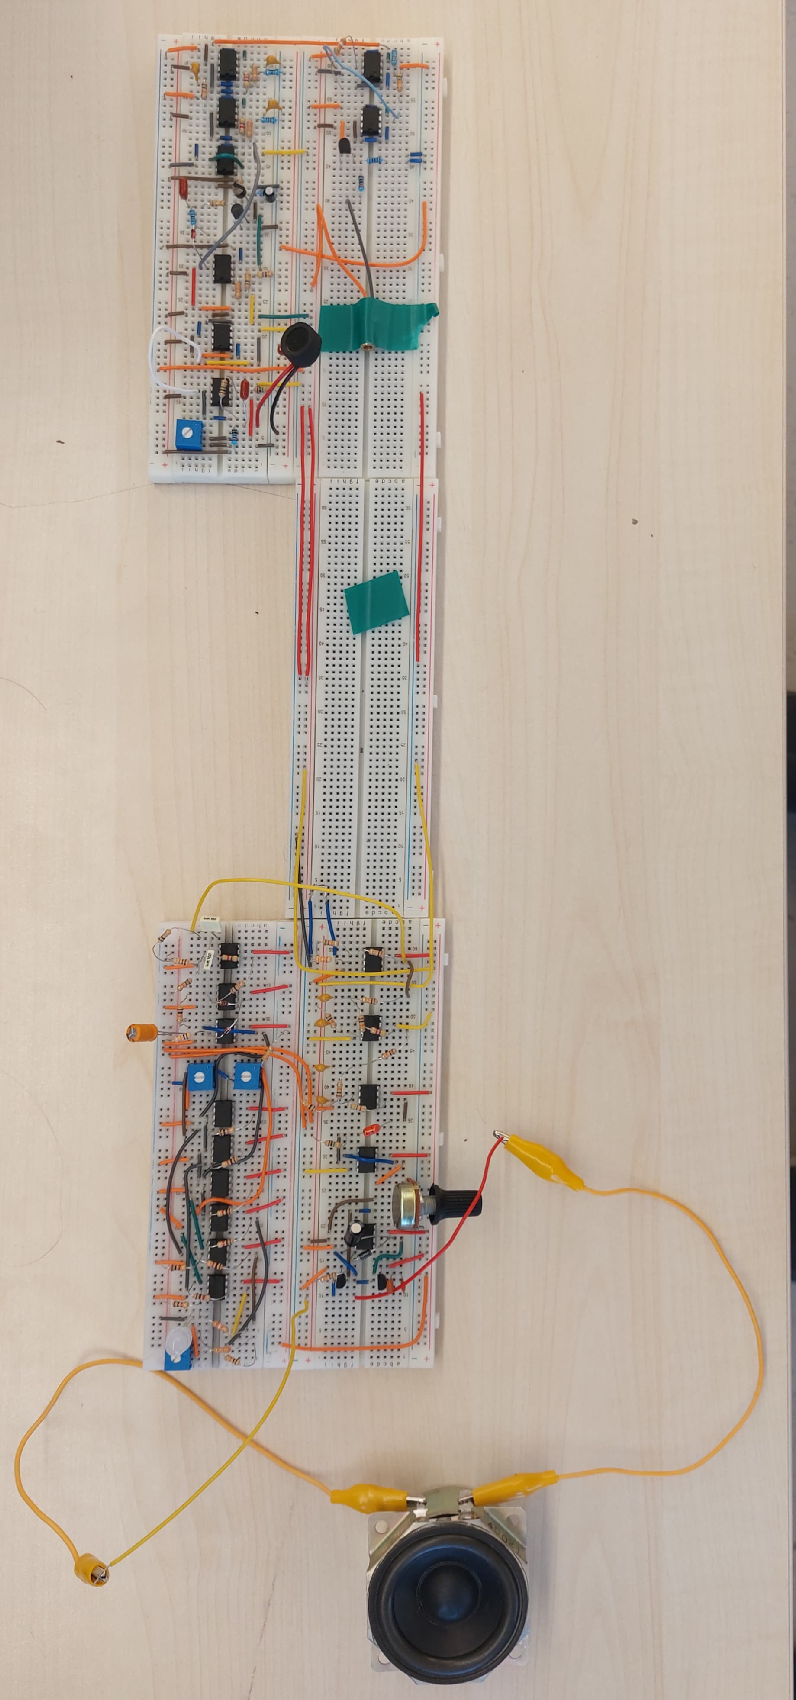
\includegraphics[scale=0.3]{all.png}
    \caption{This is a wide figure that spans both columns.}
    \label{fig:img1}
\end{figure}

\begin{figure}[H]
    \centering
    \includesvg[inkscapelatex=false, scale=0.5]{all_circuit}
    \caption{This is a wide figure that spans both columns.}
    \label{fig:img2}
\end{figure}




\bibliographystyle{ieeetr}
\bibliography{refs}
% peak detector
% https://www.analog.com/en/technical-articles/ltc6244-high-speed-peak-detector.html
% LF351 https://www.st.com/resource/en/datasheet/lf351.pdf 
% LM741 https://www.mouser.com/datasheet/2/405/snosc25c-261542.pdf
% UA741 https://www.ti.com/lit/ds/symlink/ua741.pdf
% BPW34 https://pdf.direnc.net/upload/bpw34-fotodiyot-datasheet.pdf
% https://www.electronicshub.org/butterworth-filter/
% 1N4148 https://www.vishay.com/docs/81857/1n4148.pdf 
\end{document}
